% Important: The shell-escape flag is required for the Minted package.
% Please compile this document with 'pdflatex -shell-escape main.tex'.
% If you are using another IDE, you may be able to specify this in the
% options or to provide an option like '% !TEX option = -shell-escape'
% in this file, depending on your builder. See the README.md for more.

% Don't put any content in here.
% Don't even include content files by using \input or \inlcude.
% Put your content into components/text.tex or include it there using \input.
% You probably want to modify the following files:
%   components/info.tex             contains the author, title etc.
%   components/settings.tex         contains the packages and settings.
%   components/commands.tex         contains helpful custom commands.
%   components/glossary.tex         contains an explanation of the used terms.
%   components/acknowledgements.tex contains the acknowledgements.
%   components/quote.tex            contains a quote.
%   components/abstract.tex         contains the abstract of the document.
%   components/text.tex             includes the actual content of the document.
%   components/outline.tex          contains the outline.
%   components/preface.tex          contains the preface.
%   chapters/                       contains the main text.
%   bibliography/literature.bib     contains the BibTeX entries.
%   images/                         contains all your content-related images.
%
% You probably don't need to change anything in the following files:
%   components/cover.tex            formats the front cover of the document.
%   components/titlepage.tex        formats the title page of the document.
%   components/disclaimer.tex       formats the disclaimer page.
%   styles/                         contains style elements (e.g. logos).
%   main.tex                        contains the top-level code structure.
%   README.md                       contains information about this template.

\documentclass[11pt,
              a4paper,
              article,
              index=totoc,
              headsepline,
              footsepline,
              BCOR=12mm,
              dvipsnames,
              DIV=13]{scrbook}
\setcounter{secnumdepth}{3}
\usepackage{amsthm}
\usepackage[ruled,vlined]{algorithm2e}
\usepackage{tikz}
\usepackage{wrapfig}
\usetikzlibrary{shapes,arrows,positioning}
\setlength{\parindent}{0pt}
\setlength{\parskip}{6pt}
\usepackage{caption}
\usepackage{subcaption}
\usepackage{adjustbox}
\usepackage{acronym}
\usepackage{hyperref}[2011/02/05]

\makeatletter
\AtBeginDocument{%
  \renewcommand*{\AC@hyperlink}[2]{#2}%
}
\makeatother

% KOMA scrbook options:
%  index=totoc: include an entry for the index in the table of contents.
%  headsepline: use horizontal line under heading.
%  footsepline: use horizontal line above footer.
%  BCOR: binding correction (e.g.: BCOR=12mm)
%  DIV: Number of sheet sections (used for layout) (e.g.: DIV=13)


%  This code base is currently hosted at: 
%  https://github.com/waltsims/TUM_Thesis_Template_CSE
\usepackage[backend=biber, sorting=none]{biblatex}
\addbibresource{bibliography/literature.bib}
% !TEX root = ../main.tex
% Set here the title, authors and other stuff to be used for the cover
% This file is used by MAIN.TEX

% set title, authors and stuff for the cover
\def\university{Technical University of Munich}
\def\department{School of Computation, Information and Technology - Informatics}
\def\universityLogo{styles/tum_logo}
\def\program{Robotics, Cognition, Intelligence (M.Sc.)}
\def\programLogo{styles/cse_logo}
\def\doctype{Master's Thesis in Robotics, Cognition, Intelligence}

\def\title{Active Critic in Partially Observable Markov Decision Processes}
\def\titleger{Aktiver Kritiker in teilweise beobachtbaren Markov-Entscheidungsprozessen}
\def\author{Hendrik Elvers}
\def\supervisor{Prof. Dr.-Ing. habil. Alois Knoll}
\def\advisor{Dr. rer. nat. Zhenshan Bing}
\def\date{April 15th, 2023}

\def\keywords{{RL}, {IL}, {POMDP}, {MDP}}

% The following are used for the PDF metadata, by default the same as above.
\def\metaTitle{\title}
\def\metaAuthor{\author}
\def\metaSubject{\doctype\ -\ \university}
\def\metaKeywords{\keywords}

% text to appear in the footer
\def\footertext{}


\input{components/settings}

\input{components/commands}

\input{components/glossary}

\makeglossaries

\begin{document} 

\begin{figure}
    \centering
    \begin{tikzpicture}
        \node[draw, fill=black!20, rounded corners, minimum width=2cm, minimum height=1cm] (planner) at (3,0) {$\text{Planner}_{t\rightarrow \color{black!50!green!80} t+1}$};
        \node[draw, fill=black!20, rounded corners, minimum width=2cm, minimum height=1cm] (critic) at (6,2) {Critic};
        \node[draw, fill=black!20, rounded corners, minimum width=2cm, minimum height=1cm] (actor) at (0,2) {$\text{Actor}_{t\rightarrow \color{black!50!green!80} t+1}$};
        
        \node[draw, fill=blue!20, rounded corners] (plans) at (0,0) {
            $\begin{cases}
                \begin{matrix}[p_1, ..., p_T\end{matrix} ]^\textbf{T}_{t>1}\\
                [0]_{t=1}
            \end{cases}$
            };
        \node[draw, fill=blue!20, rounded corners] (actions) at (3,2) {$\left[\begin{matrix}a_1\\ \vdots\\ a_T\end{matrix}\right]_t$};
        \node[draw, fill=blue!20, rounded corners] (exp_values) at (8.5,2) {$\left[\begin{matrix}c_1\\ \vdots\\ c_T\end{matrix}\right]_t$};
        \node[draw, thick, rectangle] (loss) at (11,2) {$|c^t_T - 1|_{_2}^{^2}$};

        \node[draw, fill=blue!20, rounded corners] (obs_1) at (0,5) {$\begin{matrix}[o_1,..., \times T, ..., o_1\end{matrix} ]^\textbf{T}$};
        \node[draw, fill=blue!20, rounded corners] (obs_2) at (6,5) {$\begin{matrix}[o_1,..., \times T, ..., o_1\end{matrix} ]^\textbf{T}$};

        \node[draw, thick, circle] (embplus_1) at (0,3.5) {$\oplus$};
        \node[draw, thick, circle] (embplus_2) at (6,3.5) {$\oplus$};

        \node[draw, thick, circle, inner sep=0pt,label={[align=left]left:Positional\\Encoding}] 
        (pe_1) at (-1.5,3.5) {\tikz \draw[scale=0.1] plot[domain=0.0:6.28] (\x,{sin(\x r)});};
        \node[draw, thick, circle, inner sep=0pt,label={[align=left]left:Positional\\Encoding}] 
        (pe_2) at (4.5,3.5) {\tikz \draw[scale=0.1] plot[domain=0.0:6.28] (\x,{sin(\x r)});};


        \draw[<-, black!50, line width=1pt] (plans)  to (planner);

        \draw[->, black!50, line width=1pt] (plans)  to (actor);

        \draw[->, black!50, line width=1pt] (actor) to (actions);
        \draw[->, black!50!green!50, line width=1pt, bend right = 30, dashed] (actions.west) to (actor.east);

        \draw[->, black!50, line width=1pt] (critic) to (exp_values);
        \draw[->, black!50!green!50, line width=1pt, bend right = 30, dashed] (exp_values.west) to (critic.east);

        \draw[->, black!50, line width=1pt] (actions) to (critic);
        \draw[->, black!50!green!50, line width=1pt, bend right = 30, dashed] (critic.west) to (actions.east);

        \draw[->, black!50, line width=1pt] (obs_1) to (embplus_1);
        \draw[->, black!50, line width=1pt] (embplus_1) to (actor);
        \draw[->, black!50, line width=1pt] (actions) to (planner);
        \draw[->, black!50!green!50, line width=1pt, bend right = 30, dashed] (actions.south) to (planner.north);


        \draw[->, black!50, line width=1pt] (pe_1) to (embplus_1);

        \draw[->, black!50, line width=1pt] (embplus_2) to (critic);
        \draw[->, black!50, line width=1pt] (obs_2) to (embplus_2);
        \draw[->, black!50, line width=1pt] (pe_2) to (embplus_2);

        \draw[->, black!50, line width=1pt] (exp_values) to (loss);
        \draw[->, black!50!green!50, line width=1pt, bend right = 30, dashed] (loss.west) to (exp_values.east);


    \end{tikzpicture}
\caption*{Overview of the inference AVC.}
\label{fig:inference}

\end{figure}


\begin{figure}
    \centering
    \begin{tikzpicture}
        \node[draw, fill=black!20, rounded corners, minimum width=2cm, minimum height=1cm] (planner) at (3,0) {$\text{Planner}_{t\rightarrow \color{black!50!green!80} t+1}$};
        \node[draw, fill=black!20, rounded corners, minimum width=2cm, minimum height=1cm] (critic) at (6,2) {Critic};
        \node[draw, fill=black!20, rounded corners, minimum width=2cm, minimum height=1cm] (actor) at (0,2) {$\text{Actor}_{t\rightarrow \color{black!50!green!80} t+1}$};
        
        \node[draw, fill=blue!20, rounded corners] (plans) at (0,0) {
            $\begin{cases}
                \begin{matrix}[p_1, ..., p_T\end{matrix} ]^\textbf{T}_{t>1}\\
                [0]_{t=1}
            \end{cases}$
            };
        \node[draw, fill=blue!20, rounded corners] (actions) at (3,2) {$\left[\begin{matrix}a_1\\ \vdots\\ a_T\end{matrix}\right]_t$};
        \node[draw, fill=blue!20, rounded corners] (exp_values) at (8.5,2) {$\left[\begin{matrix}c_1\\ \vdots\\ c_T\end{matrix}\right]_t$};
        \node[draw, thick, rectangle] (loss) at (11,2) {$|c^t_T - 1|_{_2}^{^2}$};

        \node[draw, fill=blue!20, rounded corners] (obs_1) at (0,5) {$\begin{matrix}[o_1, o_2, ..., o_\mathrm{t}, o_\mathrm{f}..., o_\mathrm{f}\end{matrix} ]^\textbf{T}$};
        \node[draw, fill=blue!20, rounded corners] (obs_2) at (6,5) {$\begin{matrix}[o_1, o_2, ..., o_\mathrm{t}, o_\mathrm{f}..., o_\mathrm{f}\end{matrix} ]^\textbf{T}$};

        \node[draw, thick, circle] (embplus_1) at (0,3.5) {$\oplus$};
        \node[draw, thick, circle] (embplus_2) at (6,3.5) {$\oplus$};

        \node[draw, thick, circle, inner sep=0pt,label={[align=left]left:Positional\\Encoding}] 
        (pe_1) at (-1.5,3.5) {\tikz \draw[scale=0.1] plot[domain=0.0:6.28] (\x,{sin(\x r)});};
        \node[draw, thick, circle, inner sep=0pt,label={[align=left]left:Positional\\Encoding}] 
        (pe_2) at (4.5,3.5) {\tikz \draw[scale=0.1] plot[domain=0.0:6.28] (\x,{sin(\x r)});};


        \draw[<-, black!50, line width=1pt] (plans)  to (planner);

        \draw[->, black!50, line width=1pt] (plans)  to (actor);

        \draw[->, black!50, line width=1pt] (actor) to (actions);
        \draw[->, black!50!green!50, line width=1pt, bend right = 30, dashed] (actions.west) to (actor.east);

        \draw[->, black!50, line width=1pt] (critic) to (exp_values);
        \draw[->, black!50!green!50, line width=1pt, bend right = 30, dashed] (exp_values.west) to (critic.east);

        \draw[->, black!50, line width=1pt] (actions) to (critic);
        \draw[->, black!50!green!50, line width=1pt, bend right = 30, dashed] (critic.west) to (actions.east);

        \draw[->, black!50, line width=1pt] (obs_1) to (embplus_1);
        \draw[->, black!50, line width=1pt] (embplus_1) to (actor);
        \draw[->, black!50, line width=1pt] (actions) to (planner);
        \draw[->, black!50!green!50, line width=1pt, bend right = 30, dashed] (actions.south) to (planner.north);


        \draw[->, black!50, line width=1pt] (pe_1) to (embplus_1);

        \draw[->, black!50, line width=1pt] (embplus_2) to (critic);
        \draw[->, black!50, line width=1pt] (obs_2) to (embplus_2);
        \draw[->, black!50, line width=1pt] (pe_2) to (embplus_2);

        \draw[->, black!50, line width=1pt] (exp_values) to (loss);
        \draw[->, black!50!green!50, line width=1pt, bend right = 30, dashed] (loss.west) to (exp_values.east);


    \end{tikzpicture}
\caption*{Overview of the inference COAVC.}
\label{fig:inference}

\end{figure}

$$J(\phi, C_{\theta(\phi)}) = \mathbb{E}_{\tau \propto (s_1, a_{1:T})}\left[ \sum_{t=1}^T \gamma^t r(s_t,a_t) \right] = \mathbb{E}_{\tau \propto (s_1, a_{1:T})}\left[ \sum_{t=1}^T \gamma^t C_{\theta(\phi)}(s_1,a_{1:T})(t) \right]$$

\end{figure}

\begin{figure}[htbp]
    \centering
    \begin{subfigure}[t]{0.32\textwidth}
      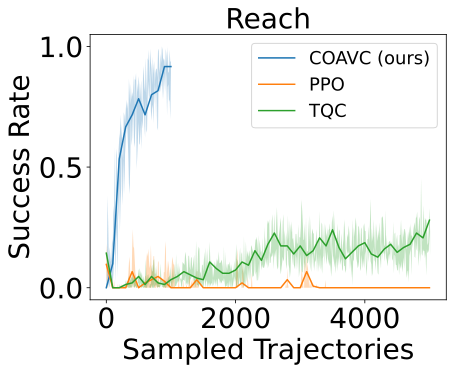
\includegraphics[width=\textwidth]{images/dense_1_big_font/Reach.png}
      \caption{One expert demonstration.}
    \end{subfigure}
    \begin{subfigure}[t]{0.32\textwidth}
      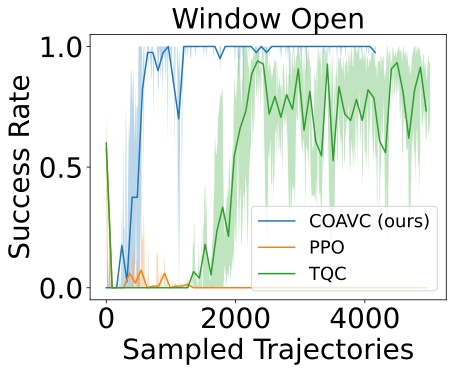
\includegraphics[width=\textwidth]{images/dense_1/Window Open.png}
      \caption{One expert demonstration.}
    \end{subfigure}
  
    \begin{subfigure}[t]{0.32\textwidth}
      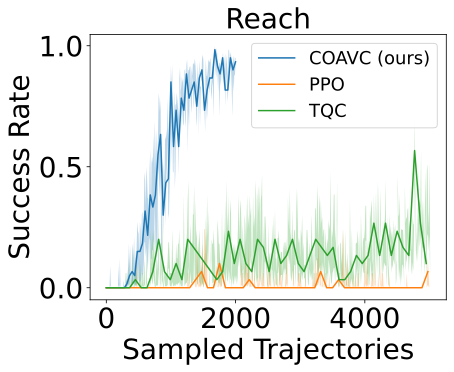
\includegraphics[width=\textwidth]{images/dense_0/Reach.png}
      \caption{No expert demonstrations.}
    \end{subfigure}
    \begin{subfigure}[t]{0.32\textwidth}
      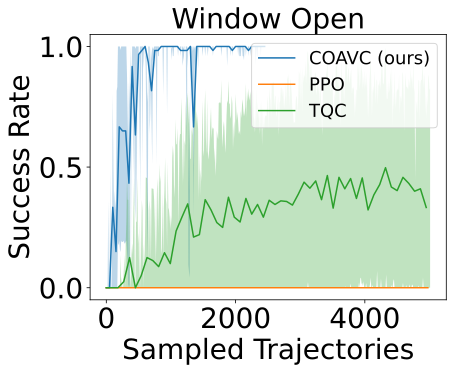
\includegraphics[width=\textwidth]{images/dense_0/Window Open.png}
      \caption{No expert demonstrations.}
    \end{subfigure}
    \begin{subfigure}[t]{0.32\textwidth}
      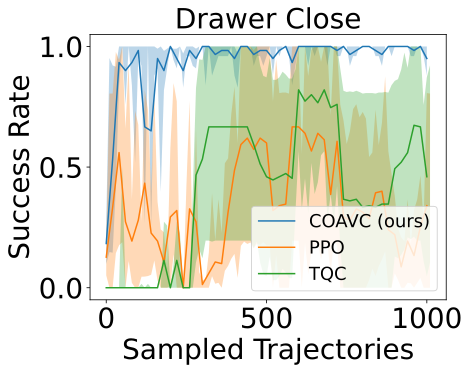
\includegraphics[width=\textwidth]{images/dense_0/Drawer Close.png}
      \caption{No expert demonstrations.}
    \end{subfigure}

  \end{figure}

  \documentclass{article}
\usepackage{tikz}

\begin{document}
    
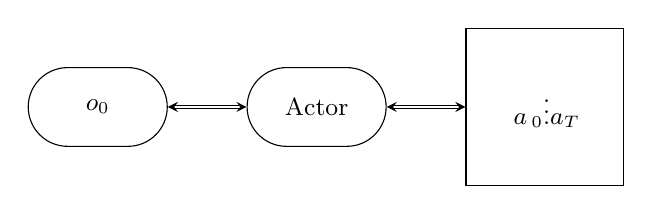
\begin{tikzpicture}[>=stealth,font=\small]
    
    % Define node styles
    \tikzstyle{block} = [draw, rounded rectangle, minimum width=2cm, minimum height=1cm, text centered]
    \tikzstyle{vector} = [draw, rectangle, minimum width=2cm, minimum height=2cm, text centered]
    
    % Draw nodes
    \node [block] (o0) {$o_0$};
    \node [block, right=1cm of o0] (actor) {Actor};
    \node [vector, right=1cm of actor] (vector) {$\begin{matrix}a_0\\ \vdots\\ a_T\end{matrix}$};
    
    % Draw arrows
    \draw [<->, double] (o0) -- (actor);
    \draw [<->, double] (actor) -- (vector);
    
\end{tikzpicture}

\end{document}

\end{document}
